\documentclass[oneside, german]{htwg-report}

% !TEX root = ../report.tex
% Use german umlaute
\usepackage{german,ngerman}
\usepackage[T1]{fontenc}
\usepackage[utf8]{inputenc}
\usepackage[ngerman]{babel}
\usepackage[autostyle=true,german=quotes]{csquotes}

%\usepackage[table]{xcolor}\usepackage{float}
%\usepackage{xcolor,colortbl}

%%\RequirePackage{amsmath}
%%\RequirePackage{amssymb}

\usepackage{epigraph}
\usepackage{gensymb}
\usepackage{float}
\usepackage{subfig}
\usepackage[backend=bibtex]{biblatex}
\addbibresource{report.bib}

\begin{document}

\pagenumbering{gobble}

%% 'reporttype' add background elements to the cover / front page
%% possible values are:
%% bachelor	--> B S C
%% master	--> M S C
%% other		--> none
\reporttype{master}
\reporttypetext{Teamprojekt}

\newcommand{\verfasserA}{Lukas Hornung}
\newcommand{\verfasserB}{Lukas Luschin}
\newcommand{\verfasserC}{Moritz Schmidt}
\newcommand{\verfasserD}{Timmo Waller-Ehrat}
\newcommand{\verfasserE}{}
\newcommand{\thema}{Mehrbildkamerasystem zur räumlichen Detektion von Modellhubschraubern}
\newcommand{\hoschschule}{Hochschule für Technik, Wirtschaft und Gestaltung}
\newcommand{\institut}{HTWG Konstanz, Institut für Optische Systeme}
\newcommand{\prueferA}{Prof. Dr. Georg Umlauf}
\newcommand{\prueferB}{Prof. Dr Matthias O. Franz}
\newcommand{\prueferC}{Dennis Griesser}


\title[Mehrbildkamerasystem zur räumlichen Detektion von Modellhubschraubern]{\thema}

\doclocation{Konstanz}
\docdate{27. Februar 2020}

\makecover[]
%          
%% Include an optional title page.
%% !TEX root = report.tex
\begin{titlepage}
\newgeometry{hscale=0.81,vscale=0.8}

\AddToShipoutPicture*{\BackgroundImgTitelPage}

\vspace*{\bigskipamount}


%% Print the title in htwg-teal.
{\makeatletter
\fboxsep=0pt
\colorbox{htwg-white}{\begin{minipage}[t]{145mm}
    \begin{center}
        %% Print Report Type Text
        \color{black}\Huge{\@report@typetext}
        \\
        %% Print Report Title
        \color{black}\Huge\textbf{\@title}
    \end{center}
\end{minipage}}
\makeatother}

\bigskip
\bigskip

{
\setlength{\parskip}{0.5cm}
\begin{center}
	\textbf{zur Erlangung des akademischen Grades}
	
	\textbf{\Large \type\ of Science (\typeshortcut. Sc.)}
	
	\textbf{an der}
	
	\textsf{\huge Hochschule Konstanz}\\
	{\small Technik, Wirtschaft und Gestaltung}
	
    \textsf{\Large Fakultät Informatik} \\
	Studiengang \studiengang
	
\end{center}
}

\bigskip
\bigskip
\bigskip

\begin{center}
	\begingroup
	\renewcommand*{\arraystretch}{1}
	\rowcolors{2}{white}{white}
	{\makeatletter
		\begin{tabular}{lll}
			\type kandidat: & \verfasser \\
							& \strasse \\
							& \wohnort \\ \\ \\ \\
	
			1. Prüfer: & \prueferA \\
			2. Prüfer: & \prueferB \\ \\ \\ \\
			
			Ausgabedatum: & \ausgabedatum \\
			Abgabedatum: & \abgabedatum
		\end{tabular}
		\makeatother}
	\endgroup
\end{center}


%% reset page margins
\newgeometry{hscale=0.7,vscale=0.8}
\end{titlepage}




% !TEX root = report.tex
\chapter*{Extended Abstract}

\begin{center}
	\begingroup
	\renewcommand*{\arraystretch}{1}
	\rowcolors{2}{white}{white}
	{\makeatletter	
		\begin{tabular}{p{3.2cm}p{9.6cm}}
			Thema: & \thema \\
			& \\
			Teammitglieder: & \verfasserA, \verfasserB, 
			\verfasserC, \verfasserD\\
			& \\
			Betreuer: & \hoschschule \newline \institut \newline \prueferA, \prueferB \\
			& \\
		\end{tabular}
		
		\makeatother}
	\endgroup
\end{center}

\bigskip

\noindent
Unser Projekt behandelt das r"aumliche Detektieren eines Modellhubschraubers. Die Detektion soll unter Laborbedingungen, das hei"st, der Helikopter befindet sich vor einer wei"sen Wand, stattfinden. Mittels der Detektion soll auf einem Bild angezeigt werden, wo sich der Mittelpunkt des Helikopters befindet. Auch die Tiefe (Entfernung zur Kamera) des Helikopters soll ermittelt werden. F"ur diese Detektion sollen zwei oder mehr Kameras verwendet werden. Bei diesen handelt es sich um HIERKAMERAEINF"UGEN, die mit dem Computer "uber ein FireWire-Kabel verbunden sind.\newline

\begin{figure}[H]
	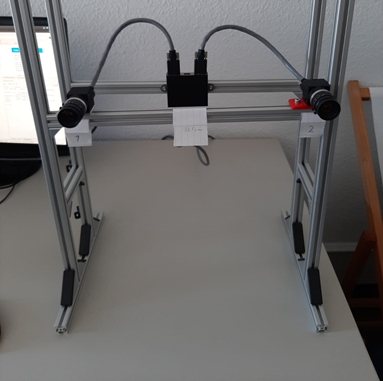
\includegraphics[scale=1.0]{bilder/camerasystem}
	\caption[Kamera-System]{Kamera-System}
\end{figure}

\noindent Das Projekt wurde erfolgreich umgesetzt.
Mittels zwei Kameras, die auf einer geraden Linie angebracht sind, kann der Mittelpunkt des Helikopters und dessen Abstand zur Kamera ermittelt werden.\newline
Unser Programm kalibriert als erstes die Kameras einzeln und anschlie"send zu einander. Das Kalibrieren erfolgt "uber ein Schachbrett-Muster. Sind die Kameras zueinander kalibriert, kann mittels eines Feature-Detektors eine Punktewolke des Helikopters generiert und der Mittelpunkt berechnet werden.

\begin{figure}%
	\centering
	\subfloat[Kamera-Kalibrierung]{{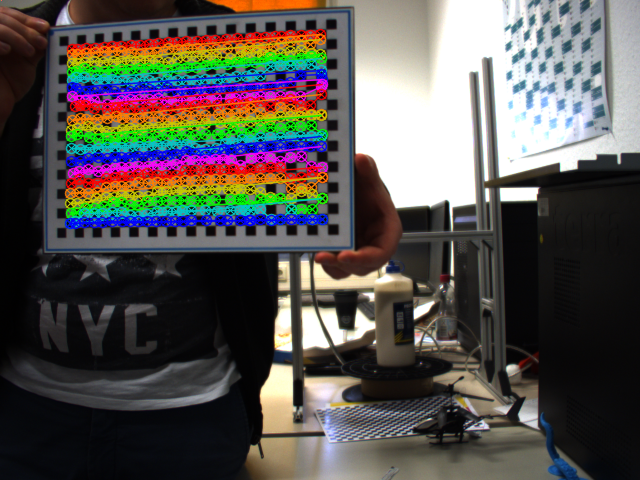
\includegraphics[width=6cm]{bilder/calibration} }}%
	\qquad
	\subfloat[Helikopter-Punktewolke]{{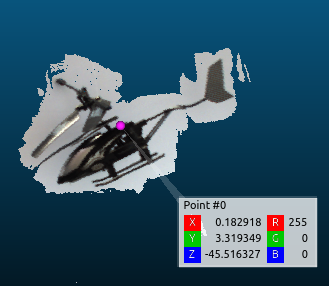
\includegraphics[width=6cm]{bilder/helicloud} }}%
	\caption{Kamera-Kalibrierung und Punktewolke}%
	\label{fig:example}%
\end{figure}
\noindent Eine m"ogliche Erweiterung des Projekts w"are das Kalibrieren von zwei Stereo-Systemen zu einander, um eine noch h"ohere Genauigkeit zu erlangen. Dies wurde versucht umzusetzen, ist allerdings gescheitert.


% !TEX root = report.tex
\chapter*{Abstract}
Ziel des Projekts war das r"aumliche Detektieren eines Modellhubschraubers. Die Detektion soll unter Laborbedingungen stattfinden. Das hei"st, der Helikopter befindet sich vor einer wei"sen Wand.
Zur Lokalisierung des Helikopters im Raum soll zun"achst eine 3D-Punktewolke der Szene generiert und daraus mit Hilfe des Clustering-Algorithmus k-Means die Position des Helikopters bestimmt werden. Auch die Tiefe (Entfernung zur Kamera) des Helikopters soll ermittelt werden. Die Detektion soll mit Hilfe von zwei oder mehr Kameras des Herstellers Point Grey, die "uber eine FireWire-Schnittstelle mit einem Computer verbunden sind, stattfinden.

\tableofcontents
\newpage
\chapter{Einleitung}
\label{cha:einleitung}

\section{Aufgabenstellung und Zielsetzung}
\label {sec:aufgabenstellungzielsetzung}

Im Rahmen dieses Teamprojekts stand die Entwicklung eines Mehrbildkamerasystems zur r"aumlichen Detektion eines Modellhubschraubers. Dies beinhaltet sowohl das Erkennen des Helikopters, als auch die Abstandsmessung von diesem. Dies sollte mit Hilfe von Bilderverarbeitungs- und Machine Learning-Techniken, sowie der Verwendung von zwei oder mehr Kameras umgesetzt werden.\newline
Die Lernziele umfassten das Erlernen des Umgangs mit Kameras f"ur die industrielle Bildverarbeitung, sowie ein Verst"andnis f"ur die Grundlagen industrieller Signalverarbeitung zu schaffen. Zudem sollten grundlegende KI-Verfahren erlernt werden.

\newpage

\section{Motivation}
\label {sec:motivation}

\setlength\epigraphwidth{15cm}
\setlength\epigraphrule{0pt}

\epigraph{\textit{\glqq Computer vision, or the ability of artificially intelligent systems to see like humans, has been a subject of increasing interest and rigorous research for decades now.\grqq{}}}{--- \textup{}Naveen Joshi\cite{NJ}\\}

\noindent Das maschinelle Sehen gewinnt in den letzten Jahren immer mehr an Popularit"at. Sei es in der Forschung oder z.B. in der Spieleentwicklung f"ur Augmented Reality. Durch die steigende Relevanz in der Praxis wurde auch unser Interesse f"ur dieses Themengebiet geweckt. Es ist spannend zu verstehen, wie komplex die Dinge, die f"ur uns Menschen selbstverst"andlich erscheinen, wie zum Beispiel das r"aumliche Sehen, eigentlich sind.
Ein weiterer Anreiz f"ur das Projekt waren die verschiedenen angewandten Technologien. Wir alle interessieren uns sehr f"ur das Programmieren. Viel Erfahrung in der Programmiersprache Python hatte aber anfangs keines der Teammitglieder. Somit war das Erlernen dieser Sprache eine weitere Motivation.\newline
Auch die zum Gro"steil verwendete und weit verbreitete Bibliothek f"ur Computer Vision-Anwendungen in Python ''OpenCV'' hat das Interesse an dem Projekt geweckt.

\section{Aufbau}
\label {sec:aufbau}
Die Ausarbeitung des Teamprojekts besteht aus drei Teilen.\newline
Anfangs wird kurz auf die angewandten Technologien eingegangen.
Anschlie"send wird die eigentliche Umsetzung und das Vorgehen erl"autert. Zuletzt wird auf die aufgetretenen Probleme eingegangen und ein Fazit gezogen.

\chapter{Projektplan}
\label{cha:projektplan}

Das Arbeiten in einem Team, indem es keine Hierarchie geben soll, ist verbunden mit agilem Entwickeln. Wichtig f"ur keine strenge Rolleneinteilungen ist die permanente Dokumentation und das verständliche Entwickeln, damit die Weiterentwicklung von allen Teammitgliedern zu jeder Zeit möglich ist. Die Kommunikation der Mitglieder und der Austausch von neu erlerntem Wissen funktionierten azyklisch. Terminierte Treffen wurden einberufen um unsere Fortschritte zu besprechen und neue Anforderungen des Projektbetreuers zu bekommen. Einen Zeitplan mit einigen Meilensteine, haben wir nach der ersten Einarbeitungsphase erstellt. Anhand von diesem können wir gut unsere Fortschritte und unsere Misserfolge darstellen. Die Anpassung der Zwischenschritte wird in Kapitel Probleme genauer dargestellt.\newline
Die Abbildung \ref{ms1} zeigt den genaueren Zeitplan, mit mehreren Arbeitspaketen, welche einen Zeiteinschätzung haben und an denen man erkennen kann welche Pakete von welchen Abhängen. Die Zwischenziele sind als Meilensteine aufgetragen. Das erfolgreiche Abschließen der Arbeitspakete und Meilensteine wurde bis zum Zwischentermin abgeschlossen. Die Einarbeitungsphase und die Lieferung der Hardware haben viel Zeit eingenommen, werden aber nicht weiter thematisiert. Bis zur Zwischenpräsentation sollten das wichtige Arbeitspaket der Kamerakalibrierung abgeschlossen sein. Des Weiteren sollte die Generierung der Punktewolke stattfinden

\begin{figure}[H]
	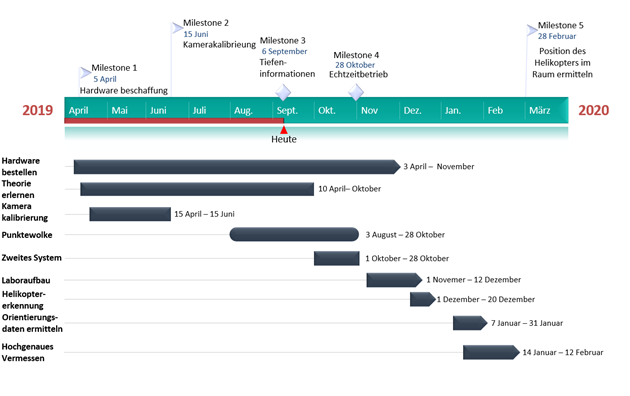
\includegraphics[scale=0.36]{bilder/ms1}
	\caption[Projektplan Zwischenergebnis]{Projektplan Zwischenergebnis}
	\label{fig:ms1}
\end{figure}

\noindent In dem endgültigen Plan mussten einige Anpassungen getroffen werden. Dies ist in der Abbildung \ref{fig:ms2} rot markiert. Der nicht eingehaltene Meilenstein 4: Echtzeitbetrieb, wurde vorerst verschoben und dann als nicht relevant für die Aufgabenstellung und die Algorithmus Entwicklung beschlossen. Das Arbeitspaket Kamerakalibrierung hat sich sehr in die Länge gezogen und ist auch noch präsent bei dem Abschluss des Projektes. Sie führt immer wieder zu Ungenauigkeiten und wird im Kapitel Probleme behandelt. Das Arbeitspaket Orientierungsdaten ermitteln, wurde in der Art geändert, dass der Helikopter erkannt wird aber nicht in seiner Ausrichtung im Raum. Die Bearbeitung nach unserem Projektplan hat zu einem Ergebnis geführt, das in den nächsten Kapiteln dargestellt wird. 

\begin{figure}[H]
	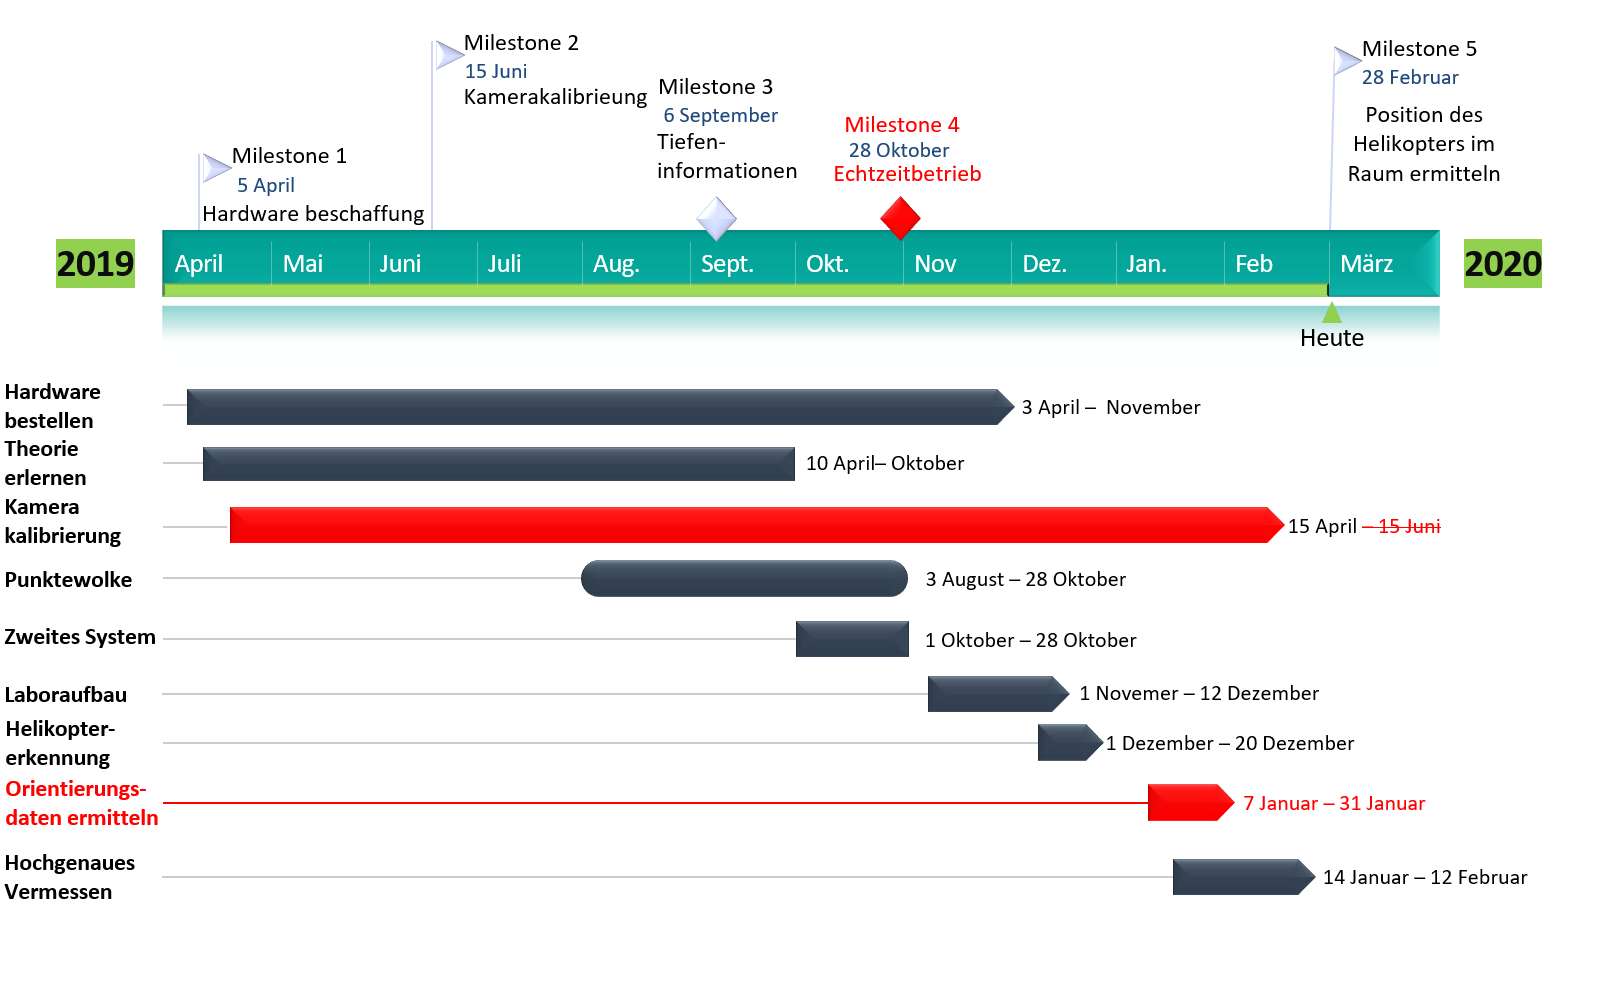
\includegraphics[scale=0.36]{bilder/ms2}
	\caption[Endgültiger Zeitplan ]{Endgültiger Zeitplan }
	\label{fig:ms2}
\end{figure}
\input{Technologien}
\chapter{Bildverarbeitung und Umsetzung}
\label{cha:verarbeitungumsetzung}

\section{Kalibrierung}
\label{sec:kalibrierung}

F"ur eine Messung, bei der der Fehler minimiert werden soll, ist das Kalibrieren der Kameras unumg"anglich. Durch die Linse einer Kamera entsteht eine tonnenf"ormige Verzeichnung. Diese Fehler sind meist so klein, dass sie vom menschlichen Auge nicht erfasst werden k"onnen \cite{VZ} \cite{VZ1}. Durch die Kalibrierung der Kamera k"onnen diese kompensiert werden.\newline

\begin{figure}[H]
	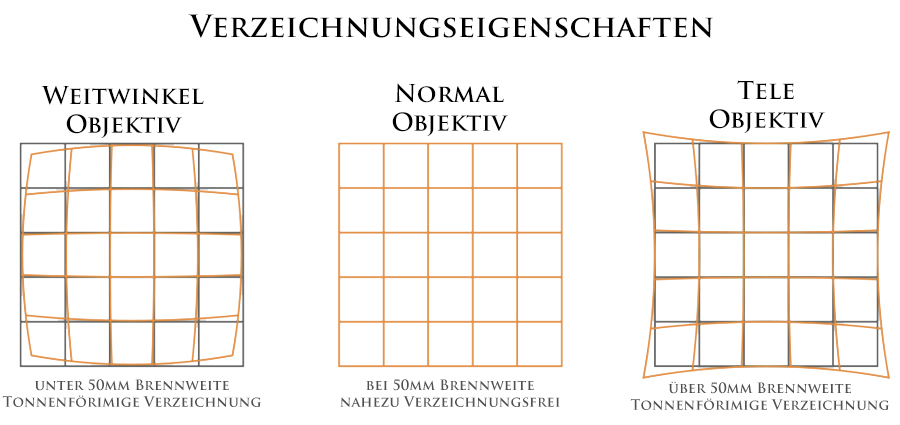
\includegraphics[scale=0.45]{bilder/verzeichnung}
	\caption[Verzeichnung]{Verzeichnung}
	\small Quelle: \url{http://www.fotokurs-bremen.de/wp-content/uploads/2016/11/Objektiv-Verzeichnung.jpg}
\end{figure}

\noindent Durch die Kamerakalibrierung werden folgende Parameter bestimmt:

\begin{description}
	\item[Intrinsische Parameter]
	Bezeichnen die Abbildung von 3D-Punkten im Kamerakoordinatensystem auf den 2D-Sensor der Kamera. Es sind Informationen der Kamera selbst, die unabh"angig davon sind, wo sich die Kamera befindet und wie diese ausgerichtet ist \cite{Intr}.
	
	\item[Extrinsische Parameter]
	Die r"aumliche Lage und Orientierung der Kamera zu einem Referenzkoordinatensystem, d.h. die Rotation und Translation \cite{cal} \cite{extr}.
\end{description}

\noindent Da es ich bei dem System um ein Stereokamera-System handelt, ist die Kalibrierung von diesem etwas komplizierter.\newline
Zuerst m"ussen die Kameras gesondert kalibriert werden. Dies wird mit der Funktion \textit{calibrateCamera} von OpenCV durchgef"uhrt. F"ur die Kalibrierung wird ein Schachbrett-Muster verwendet. Wichtig ist, dass bei der Kalibrierung beide Kameras dasselbe Bild verwenden. F"ur die Erkennung des Schachbretts wird die OpenCV-Funktion \textit{findChessboardCorners} verwendet. Diese liefert die Objekt- und Bild-Punkte der Aufnahme. Bei den Objekt-Punkten handelt es sich um die 3D-Punkte des Bildes, bei den Bild-Punkten um die 2D-Punkte \cite{OcvD}.

\begin{figure}[H]
	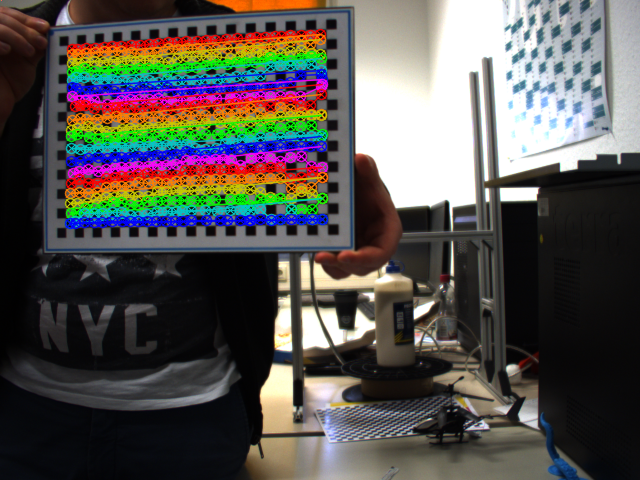
\includegraphics[scale=0.4]{bilder/calibration}
	\caption[Kalibrierung]{Kalibrierung}
\end{figure}

\noindent F"ur eine m"oglichst genaue Kalibrierung werden 50 Bilder verwendet. Anhand dieser wird jede Kamera mittels \textit{calibrateCamera} kalibriert.\newline
Die Funktion liefert die intrinsisches Parameter in Form von einer $3x3$ Kamera-Matrix

\begin{figure}[H]
	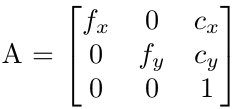
\includegraphics[scale=0.75]{bilder/matrix}
\end{figure}

\newpage

\noindent Wobei $f_{x}$ und $f_{y}$ die Brennweite in Pixeln und $c_{x}$ $c_{y}$ ein Hauptpunkt, der normalerweise in der Bildmitte liegt, ist.

\noindent Die Ergebnisse dieses Vorgangs werden auf dem Computer gespeichert, sodass dieser nicht wiederholt werden muss. Anschlie"send wird das Ergebnis der Kalibrierungen an die OpenCV-Funktion \textit{stereoCalibrate} "ubergeben.\newline
Mit Hilfe der Stereo-Kalibrierung kann der Zusammenhang zwischen den Kameras ermittelt werden: Es werden von dem Bezugsbild, welches zum Ursprung des Koordinatensystems wird, die Objekt-Punkte verwendet. Von beiden Kamerasystem werden die Bild-Punkte, die jeweiligen Kameramatrizen und die Verzeichnungskoeffizienten verwenden.

\section{Tiefeninformationen}
\label{sec:tiefeninformationen}

\noindent Das Verwenden des Stereo-Kameras ist relevant f"ur die Berechnung von Tiefeninformationen. Da die Information der Tiefe nicht in einem einzigen Bild ermittelt werden kann, wird eine zweite Kamera hinzugef"ugt. Diese ist im Raum verschoben, fotografiert aber zum gr"o"sten Teil die gleiche Szene.

\begin{figure}%
	\centering
	\subfloat[Stereosystem]{{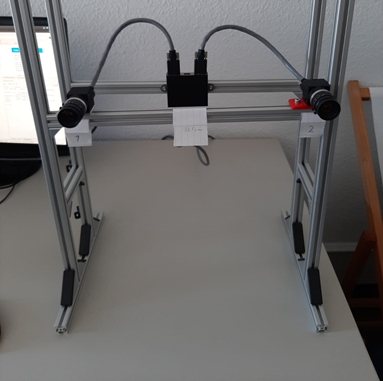
\includegraphics[width=6cm]{bilder/camerasystem} }}%
	\qquad
	\subfloat[Szenenaufnahme]{{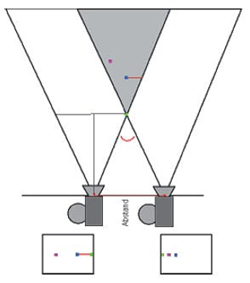
\includegraphics[width=6cm]{bilder/szene} }}%
	\caption{Stereo-System}%
	\small Quelle: \url{https://me.efi.th-nuernberg.de/interaktion/index.php5/Bearbeitung_und_Gewinnung_von_Tiefeninformation_durch_die_Kopplung_zweier_Kameras}
	\label{fig:stereo}%
\end{figure}

\noindent in \ref{fig:stereo}, im rechten Bild, ist in grau der Ausschnitt zu sehen, der von beiden Kameras erfasst wird. Das Bild daneben zeigt den Versuchsaufbau: zwei Kameras, die horizontal verschoben sind. Somit erhalten wir den Normalfall, der wie folgt beschrieben wird: \textit{Das achsparallele Stereosystem zeichnet sich durch zwei Kameras aus, die nur horizontal verschoben und deren Koordinatensysteme nicht gegeneinander verdreht sind \cite{Tu}.}\newline
\noindent Nun ist es m"oglich, "uber die Ungleichheiten des "uberlappenden Bildbereichs Tiefeninformationen zu ermitteln. Diese wird mit Hilfe der Disparit"at berechnet.\newline
Der horizontale Abstand, des gleichen Merkmals in beiden Bildern nennt man Disparit"at. \textit{Die Disparität ist umgekehrt proportional zur Tiefe. \cite{Tu}.}\newline
Durch die achsparallele Anordnung der Kameras, die nicht gegeneinander verdreht ist, kann die Z-Koordinate "uber die bekannten Kameraparameter, die Brennweite $f$ der Kameras und der Basisl"ange $B$ (Translation der Kameras zueinander), sowie die Disparit"at $D$ bestimmt werden. $D$ wird wie in \ref{fig:base} schematisch dargestellt, durch die Bildpunktverschiebung der Beiden Punkte $x$ un $x'$ berechnet. Der Z-Achsenwert berechnet sich mit der Formel $Z=\frac{f*B}{x-x'}$
 
 \begin{figure}[H]
 	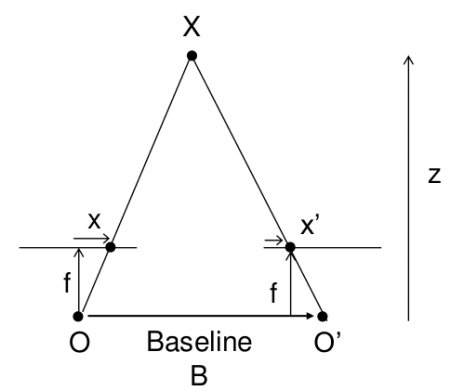
\includegraphics[scale=1.0]{bilder/tiefenberechnung}
 	\caption[Tiefenberechnung]{Tiefenberechnung}
 	\small Quelle: \url{https://opencv-python-tutroals.readthedocs.io/en/latest/py_tutorials/py_calib3d/py_depthmap/py_depthmap.html}
 	\label{fig:base}%
 \end{figure}
 
\newpage

Diese Funktion kalibriert die beiden Kameras zueinander. Dies geschieht mit Hilfe der vorher berechneten Kameramatrizen, Verzeichnungen und der Objekt- und Bild-Punkte.\newline 
Die wichtigsten Ergebnisse der Stereo-Kalibrierung sind die Rotation und die Translation der beiden Kameras zueinander.

\subsection{Fehler"uberpr"ufung}
\label{sec:fehlertest}

\section{Tiefeninformationen}
\label{sec:tiefeninformationen}

Um Tiefeninformationen aus zwei Bildern zu gewinnen, m"ussen diese zuerst rektifiziert und entzerrt werden. 

\chapter{Experimente}
\label{cha:experimente}

\section{Vereinfachte Kalibrierung}
\label{sec:vereinfachtekalib}

Eine andere M"oglichkeit, als die Kalibrierung mittels eines Schachbretts, wie sie in \ref{sec:kalibrierung} erl"autert wurde, ist mit Hilfe eines rechteckigen Kalibrierobjektes. In unserem Fall handelt es sich, wie in \ref{fig:klammern} zu sehen ist, um die Verpackung von Heftklammern.
 
\begin{figure}[H]
	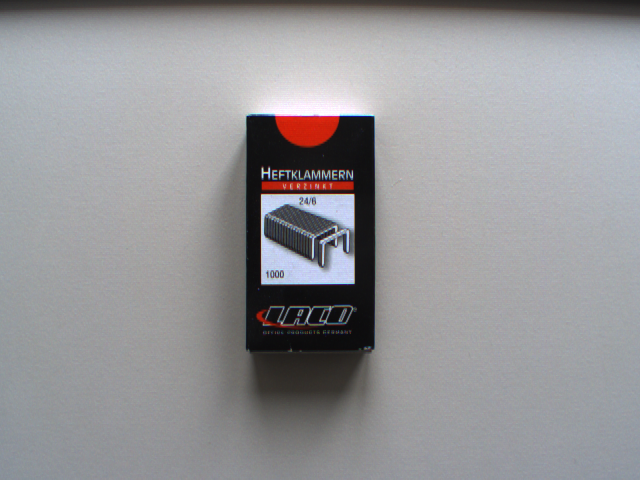
\includegraphics[scale=0.5]{bilder/experimentcalib}
	\caption[Kalibrierobjekt]{Kalibrierobjekt}
	\label{fig:klammern}
\end{figure}

\noindent Die Formel zur Berechnung der Brennweite $f_x$ und $f_y$ ergibt sich aus den Formeln

\begin{equation}
f_x=\frac{\Delta x'}{x}z
\end{equation}

und

\begin{equation}
f_y=\frac{\Delta y'}{y}z
\end{equation}

\noindent bei $\Delta x$ und $\Delta y$ handelt es sich um die jeweiligen Seitenl"angen des Kalibrierobjekts.\newline
$\Delta x'$ und $\Delta y'$ sind die L"angen der Seiten des Kalibrierobjekts in Pixelwerten. $z$ ist der Abstand zwischen Linse und Objekt \cite{PCV} \cite{CVF}.

\begin{figure}[H]
	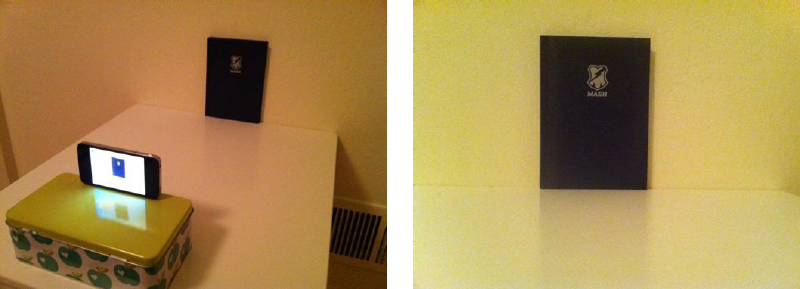
\includegraphics[scale=1.0]{bilder/simple_calib}
	\caption[Vereinfachte Kalibrierung]{Vereinfachte Kalibrierung}
	\small Quelle: Solem 2012
	\label{fig:simplecalib}%
\end{figure}

\noindent Wie in \ref{fig:simplecalib} zu sehen ist, muss das Kalibrierobjekt senkrecht auf eine plane Oberfl"ache gestellt werden. So auch die Kamera. Die Kamera muss dann so ausgerichtet werden, dass das Objekt im Bild genau zentriert und entlang der Bildzeilen und -spalten ausgerichtet ist \cite{CVF}.\newline
Obwohl diese Kalibrierung sehr ungenau erscheint, wurde ein dennoch relativ geringer Reprojection-Error errechnet. Der wie in \ref{sec:kalibrierung} ermittelte Wert war dennoch besser.

\section{Fehlerfortpflanzung}
\label{sec:fehlerfortpflanzungtiefen}

Bei der Tiefenberechnung mit Hilfe eines Stereokamerasystems wird die Raumposition nicht gemessen, sondern aus den beiden vom Kamerasystem erfassten Bildern berechnet. Dazu wird der gleiche Raumpunkt in beiden Bildern detektiert. Die räumliche Rekonstruktion ist im Stereonormalfall besonders einfach, da die beiden Kameras keine Rotation zueinander aufweisen. Dadurch vereinfachen sich die allgemeinen Formeln zur räumlichen Rekonstruktion \cite{frz}

\begin{equation}
x = x_{0} + (z - z_{0})\frac
{r_{11}(x'-x_{0}') + r_{12}(y'-y_{0}')-r_{13}f}
{r_{31}(x'-x_{0}') + r_{32}(y'-y_{0}')-r_{33}f}
\end{equation}

\begin{equation}
y = y_{0} + (z - z_{0})\frac
{r_{21}(x'-x_{0}') + r_{22}(y'-y_{0}')-r_{23}f}
{r_{31}(x'-x_{0}') + r_{32}(y'-y_{0}')-r_{33}f}
\end{equation}

\noindent zu\newline
\noindent Rechtes Bild:
\begin{equation}\label{eq:one}
x = -z \frac{x'_{1}}{f}
\end{equation}
\begin{equation}\label{eq:two}
y = -z \frac{y'_{1}}{f}
\end{equation}

\noindent Linkes Bild:
\begin{equation}\label{eq:three}
x = B-z \frac{x'_{2}}{f}
\end{equation}
\begin{equation}\label{eq:four}
y = -z \frac{y'_{2}}{f}
\end{equation}

\noindent Aus den vereinfachten Formeln \ref{eq:one}, \ref{eq:two}, \ref{eq:three} und \ref{eq:four}, ist es ersichtlich, dass ein Raumpunkt in beiden Bildern die gleiche $y$-Koordinate aufweist, sich jedoch normalerweise in der $x$-Koordinate unterscheidet. Diese Differenz wird als $x$-Parallaxe 
$\rho_{x} = x_{1} - x_{2}$ oder Disparität $D$ bezeichnet.\newline
\noindent Durch Gleichsetzen der Formeln \ref{eq:one} – \ref{eq:four} für linkes und rechtes Bild, erhält man folgende Formel zur Berechnung der Tiefeninformation:

\begin{equation}\label{eq:tiefe}
z = -\frac
{f*B}
{x'_{1}-x'_{2}}
=
-\frac
{f*B}
{\rho x'}
\end{equation}

\noindent Da die Brennweite f und der Abstand der beiden Kameras zueinander (Baseline $B$) konstant sind, ist die Entfernung allein von der $x$-Parallaxe abhängig. Dabei ist ein Punkt näher, je größer die Parallaxe ist. \newline
Die Formel \ref{eq:tiefe} wurde mit folgendem Experiment validiert:


\begin{figure}[!htb]
	\minipage{0.32\textwidth}
	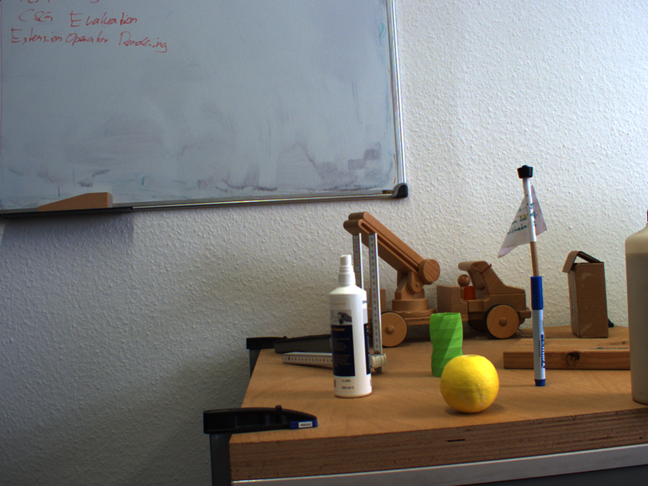
\includegraphics[width=\linewidth]{bilder/depth_left}
	\caption{Tiefe links}\label{fig:depthleft}
	\endminipage\hfill
	\minipage{0.32\textwidth}
	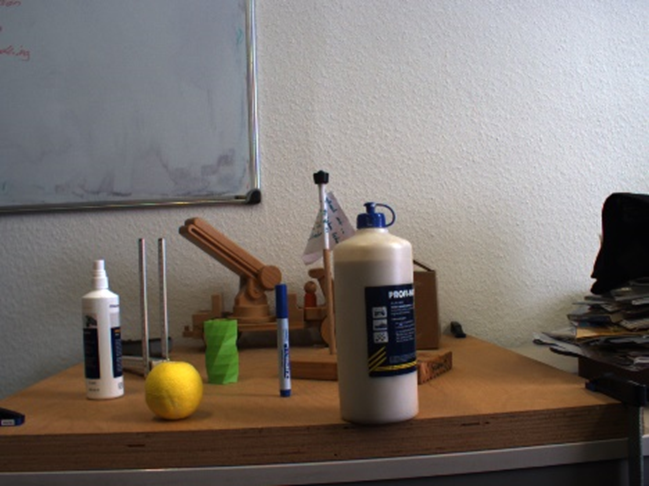
\includegraphics[width=\linewidth]{bilder/depth_right}
	\caption{Tiefe rechts}\label{fig:depthright}
	\endminipage\hfill
	\minipage{0.32\textwidth}%
	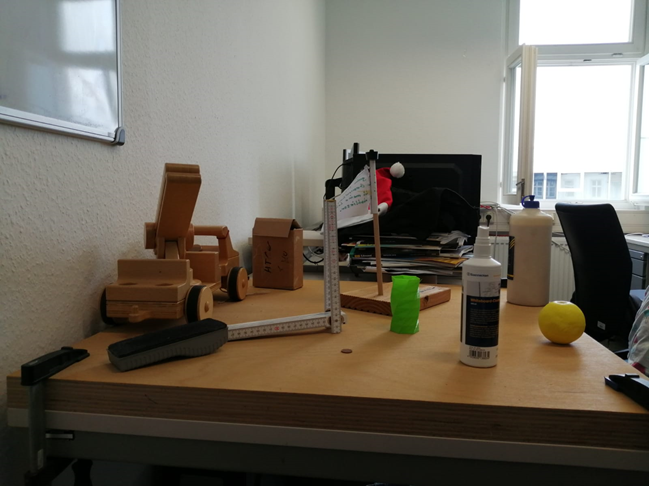
\includegraphics[width=\linewidth]{bilder/depth_side}
	\caption{Tiefe seitlich}\label{fig:depthside}
	\endminipage
\end{figure}

\noindent Mit dem Stereo-System wurden zwei Aufnahmen einer Szene aufgenommen (\ref{fig:depthleft} und \ref{fig:depthright}). Auf dem seitlichen Bild \ref{fig:depthside} sieht man die tats"achliche Tiefe der Objekte im Bild.

\begin{figure}[!htb]
	\minipage{0.48\textwidth}
	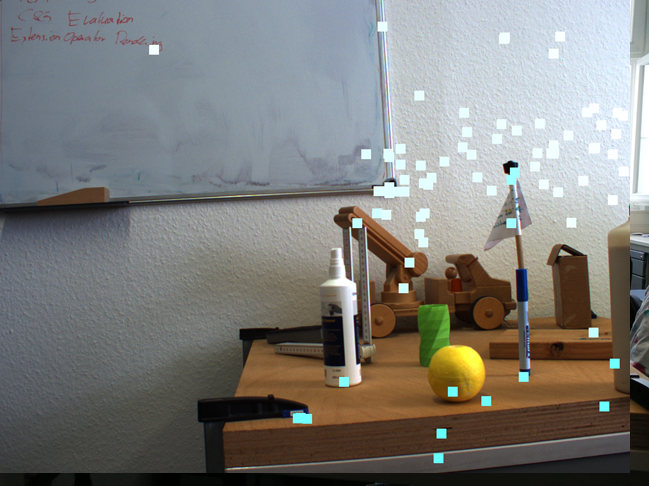
\includegraphics[width=\linewidth]{bilder/depth_result}
	\caption{Tiefeninformation Punkte}\label{fig:depthpoints}
	\endminipage\hfill
	\minipage{0.48\textwidth}
	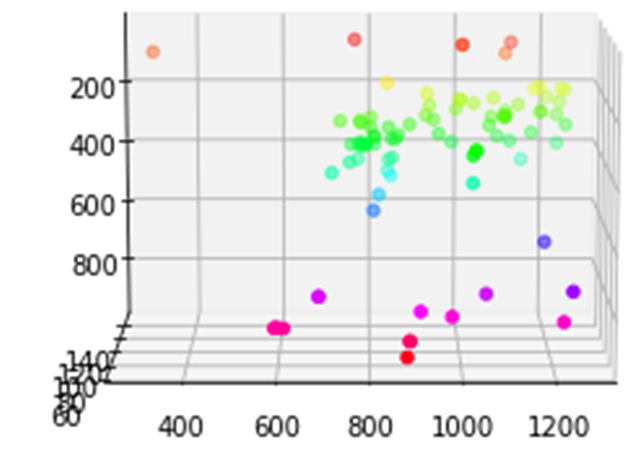
\includegraphics[width=\linewidth]{bilder/depth_coord}
	\caption{Tiefeninformation 3D-Plot}\label{fig:depthplot}
	\endminipage\hfill
\end{figure}

\noindent Auf den zwei Bildern der Szene wurden hier vorerst h"andisch, dann mittels des SIFT-Algorithmus Referenzpunkte ermittelt, zu denen die Tiefe berechnet werden sollte.\newline
\noindent Mittels eines selbst geschriebenem Algorithmus, der Werte mit großem $z$ wei"slich und Werte mit kleinem $z$ hellblau einf"arbt, kann man sich die Informationen zur Tiefe auf einem Bild darstellen. In \ref{fig:depthpoints} kann man gut erkennen, dass Objekte, die n"aher an der Kamera stehen, mit einem hellen Blau markiert sind. Objekte, die weiter entfernt sind, mit einem wei"slichem Farbton.\newline
\noindent Dieses Verfahren der indirekten Bestimmung der Tiefeninformationen ist jedoch anfällig für Messfehler in den Bildposition. Die Fehlerfortpflanzung über die Werte $x$, $y$ und $z$ wird mit Hilfe des Gaußschen Fehlerfortpflanzungsgesetzes, welches den Einfluss mehrerer fehlerbehafteter Eingangsgrößen auf eine zu schätzende Ausgangsgröße beschreibt, berechnet.
Wird die Varianz der Ausgangsgröße $y$ über die fehlerbehafteten Eingangsgrößen $x_{1}$ bis $x_{n}$  abgeschätzt, lautet die allgemeine Form des Gaußschen Fehlerfortpflanzungsgesetzes:

\begin{equation}
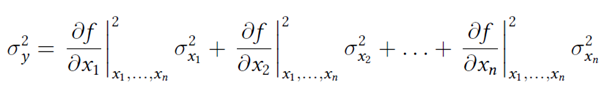
\includegraphics[scale=1.0]{bilder/formel3}
\end{equation}

\noindent Wendet man dieses Gesetz auf die Formeln \ref{eq:one} - \ref{eq:tiefe} an, erhält man folgende Fehlerabschätzung für die Größen $z$, $y$ und $z$ unter der Annahme, dass die Brennweite $f$ und die Baseline $B$ fehlerfrei sind \cite{frz}:

\begin{equation}\label{eq:fourone}
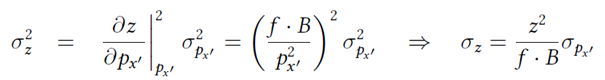
\includegraphics[scale=1.0]{bilder/fourone}
\end{equation}

\begin{equation}\label{eq:fourtwo}
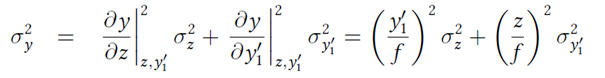
\includegraphics[scale=1.0]{bilder/fourtwo}
\end{equation}

\begin{equation}\label{eq:fourthree}
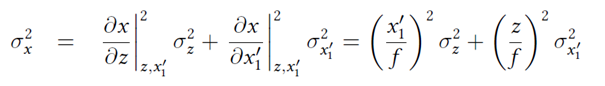
\includegraphics[scale=1.0]{bilder/fourthree}
\end{equation}


\section{Genauigkeitsabschätzung des Systems}
\label{sec:genauigkeit}

Zur Genauigkeitsbeurteilung haben wir drei Mal das gleiche Objekt in jeweils einem anderen Abstand zum Stereosystem aufgenommen. Dabei erhielten wir folgende Resultate:

\begin{center}
	\begin{tabular}{  l | l | l }
		\hline
		Gemessener Abstand [cm] & Berechneter Abstand [cm] & Differenz [cm] \\ \hline
		37 & 31,05 & 5,95 \\ \hline
		54 & 48,78 & 5,22 \\
		100 & 96,81 & 3,19 \\
	\end{tabular}
\end{center}

\noindent Überraschenderweise nimmt der Fehler mit zunehmender Distanz in diesem Fall ab. Auf Grund der Fehlerformel für $z$ (s. \ref{eq:fourone}) war zu erwarten, dass der Fehler in der Tiefe quadratisch mit der Distanz wächst, was hier jedoch nicht der Fall ist. Auch bei der händischen Tiefenberechnung mit zwei rektifizierten Schachbrettmustern trat ein Phänomen auf, wobei die Disparität von Punkten links in den beiden Bildern nach rechts stark zunahm, obwohl die Punkte in der gleichen Entfernung zur Kamera waren.\newline
\noindent Dies ist auch die Ursache, weshalb keine ausführliche Fehlerfortpflanzungsrechnung für unser System durchgeführt wurde, da bereits a priori absehbar war, wenig aussagekräftige Ergebnisse zu erhalten. Leider konnten wir keine plausible Erklärung für dieses Verhalten finden, die einzige Vermutung ist, dass etwas mit der Kalibrierung der Kameras nicht ganz in Ordnung ist, was dieses unerwartete Verhalten verursacht. Doch auch durch mehrmaliges Neukalibrieren konnte das Problem nicht behoben werden. Folgende Abbildung zeigt den Versuchsaufbau:

\begin{figure}[H]
	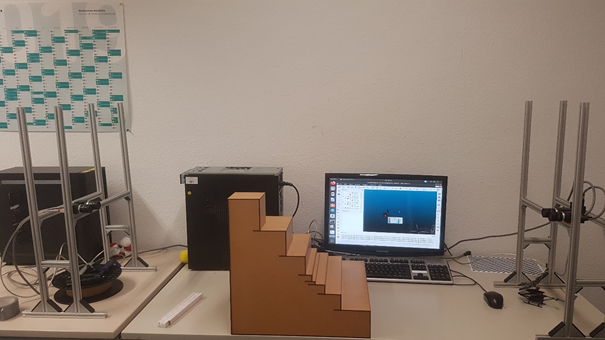
\includegraphics[scale=1.0]{bilder/abstandsmessung}
	\caption[Versuchsaufbau mit zwei Stereokamerasystemen und Objekt zur Abstandsmessung]{Versuchsaufbau mit zwei Stereokamerasystemen und Objekt zur Abstandsmessung}
	\label{fig:abstandsmessung}
\end{figure}

\section{Kalibrierung der beiden Stereokamerasysteme zueinander}
\label{sec:kalibbeide}

Durch Aufstellen eines zweiten identischen Stereokamerasystems gegenüber des bisher beschriebenen Systems (s. \ref{fig:abstandsmessung}) sollte die bisher in der generierten Punktewolke fehlende Rückansicht des Helikopters in der Punktewolke visualisiert werden. Auf diese Weise sollte also eine 360\degree \space 3D-Ansicht einer Szene generiert werden. Zunächst musste das zweite System entsprechend dem Vorgehen für das erste System kalibriert werden, bevor versucht werden konnte, die beiden System zueinander kalibrieren zu können, d.h. die Rotation und Translation der beiden Systeme zueinander zu bestimmen. Dies ist nötig, um die beiden separaten Punktewolken in ein gemeinsames Koordinatensystem überführen zu können.\newline
\noindent Zur Kalibrierung der beiden Systeme zueinander wurden mehrere verschiedene Ansätze in Betracht gezogen und getestet, um Korrespondenzpunkte im 3-dimensionalen Raum berechnen zu können. Mithilfe des Algorithmus Iterative Closest Points, welcher in \ref{sec:icp} erl"autert wird, sollten aus diesen 3D-Koordinaten die Rotation und Translation der Systeme zueinander bestimmt werden.\newline
\noindent Folgende Ansätze wurden in Betracht gezogen:

\begin{enumerate}
	\item Aufstellen eines Objektes mit mehreren Eckpunkten, die in beiden Systemen sichtbar sind mit anschließendem automatisiertem Auffinden von Korrespondenzpunkten mit Hilfe des rotationsresistenten Interest-Point-Detektors SIFT. Leider konnte der SIFT-Detektor nicht ausreichend korrekte Korrespondenzen in den beiden Aufnahmen der jeweils gewählten Referenzkameras der beiden Systeme detektieren, weshalb dieser Ansatz nicht weiterverfolgt wurde.
	
	
	\item Aufstellen eines Objektes mit mehreren Eckpunkten, die von beiden Systemen sichtbar sind. Aus den Aufnahmen sollten dann händisch die 2D-Koordinaten bestimmt und mit den Formeln 
	\ref{eq:one} - \ref{eq:four} die 3D-Repräsentation des Punkts berechnet werden. Dieser Ansatz wurde wegen des hohen manuellen Aufwands zunächst nicht weiterverfolgt und als Notlösung, falls keine bessere Variante gefunden werden könnte, verbucht. 
	
	\item Als am vielversprechendsten erwies sich der Ansatz mit einem beidseitig bedruckten Schachbrettmuster zu kalibrieren. Dabei müssen die Eckpunkte des Schachbretts auf Vorder- und Rückseite möglichst exakt übereinander liegen, dies muss bereits beim Druck berücksichtigt werden. Von dem Schachbrettmuster wird dann von beiden Systemen eine Aufnahme gemacht, diese rektifiziert und mit der aus der Kamera-Kalibrierung bereits bekannten OpenCV-Methode \textit{findChessBoardCorners} die Bildkoordinaten der Eckpunkte bestimmt. Aus diesen Bildkoordinaten können anschließend erneut mit den Formeln xyz die 3D-Koordinaten mehrerer identischer Punkte für die beiden System berechnet werden. \newline 
	\noindent Mithilfe des ICP konnten die beiden 3D-Punktewolken der beiden Schachbrettmuster auch erfolgreich in eine Ebene transformiert werden, also die Translation der beiden Systeme zueinander bestimmt werden. Problematisch war jedoch die Bestimmung der Rotation, da die Punktewolken des Schachbretts nahezu symmetrisch sind und deshalb die 180\degree-Rotation nicht erkannt wird. Eigentlich müssten die jeweils oberen linken Ecken des Schachbrettmusters aus beiden Systemen aufeinander gemappt werden. Allerdings werden durch den ICP die linke obere Ecke des Schachbrettmusters aus dem linken System auf die rechte obere Ecke der Aufnahme aus dem rechten System aufeinander gemappt, wodurch keine Rotation erkannt wird. Bei einem anderen Setup der Stereosysteme zueinander wird das Schachbrettmuster nicht mehr gleichzeitig von beiden Systemen erkannt, weshalb das Problem dadurch ebenfalls nicht gelöst werden kann.
	
\end{enumerate}

\begin{figure}[H]
	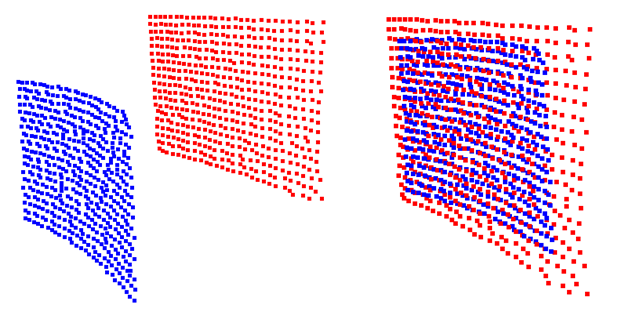
\includegraphics[scale=1.0]{bilder/icpresult}
	\caption[3D-Schachbrettmuster vor und nach der Transformation mit den Ergebnissen des ICP-Algorithmus]{3D-Schachbrettmuster vor und nach der Transformation mit den Ergebnissen des ICP-Algorithmus}
	\label{fig:icpresult}
\end{figure}

\subsection{ICP}
\label{sec:icp}

Der Iterative Closest Point Algorithmus (ICP Algorithmus) ist eine Methode um zwei Punktewolken aneinander anzupassen \cite{icp1} \cite{icp2}.
Hierzu minimiert der Algorithmus den Euklidischen Abstand $d$ von korrespondieren Punkten $q$ und $p$ in der Punktewolke:

\begin{equation}
d(q,p) = \sqrt{(q_{1}-p_{1})^{2} + ... + 
	(q_{n} -p_{n})^{2}}
\end{equation}

\noindent Die Zuordnen von Punktepaaren, um so korrespondieren Punkte zu finden, wird mittels des Nearest Neighbour Algorithmus vorgenommen. Dieser nimmt die beiden Punktewolken entgegen und liefert ein Feld mit Indizes zurück, welche die korrespondieren Punkte angeben. In unserem Projekt wird er in der optimierten Variante verwendet. Dieser beschreibt die Punktewolken in einer Baumstruktur.

\subsubsection{Ablauf}
\label{ss:ablauf}

Vorab wird angenommen, dass die Punktewolken näherungsweise aufeinander ausgerichtet wurden und als
initiale Transformation $T$ beschrieben wird. Diese Transformation wird auf die eine Punktewolke angewendet. Die daraus resultierende, wird verwendet um mit Hilfe des Nearest Neighbour Algorithmus die korrespondierenden Punktepaare zu finden. 
Als Gütemaß für die aktuelle Transformation wird die Summe der quadratischen Distanzen genommen. Diese gilt es zu minimieren. Aus diesen Ergebnissen werden dann die neuen Transformationsparameter abgeleitet \cite{icp3}:

\begin{equation}
T \leq argmin (\sum || d(q_{n}, p_{n}) || ^{2})
\end{equation}

\noindent Diese Schritte werden nun so oft wiederholt bei ein akzeptables Optimum gefunden ist. Der ICP Algorithmus terminiert also, sobald entweder ein definierter Schwellwert für das Gütemaß überschritten, oder eine definierte Anzahl an Iterationen erreicht wurde.

\chapter{Probleme}
\label{cha:probleme}

Trotz dem Erfolgreichen lokalisieren unseres Helikopters, hatten wir einige langwierigen Schwierigkeiten, die auch nicht bis zur Beendigung des Projektes gelöst wurden. Das Hauptproblem, mit dem wir nicht gerechnet hatten, war die Kalibrierung und die vielen Folgeprobleme, die sich daraus entwickelten. Nach dem Arbeitspaket Kalibrierung, in dem wir uns eingelesen, selbst kalibriert haben und unsere Methode mit den Methoden von OpenCV verglichen haben, sind wir davon ausgegangen das Thema sei abgeschlossen. Aber eine plausible Validierung aus den Daten war für uns nicht möglich. Die erhaltenen Werte konnten nicht eingeordnet werden, ob diese gut oder schlecht sind. Zwar versuchten wir immer wieder mit neuen Messungen dies zu bestätigen, aber ein konsistenter Beleg, dass unsere Kalibrierung exakt ist, war nicht möglich. So dachten wir oft wir hätten dieses Thema erfolgreich beendet, aber bei Fehlschlägen in weiterführenden Themen, wie große Unstimmigkeiten in den Resultaten, konnte durch eine exaktere Kalibrierung bessere Ergebnisse erreicht werden. Die Ergebnisse schwankten auch sehr stark, wie die Lichteinstrahlung zu Zeiten der Messung im Labor war. So war es oft am besten abends Aufnahmen zu machen, da kein direktes Licht auf unseren Versuchsaufbau fiel. Trotz des abhängen des Fensters, war es nicht möglich dieses Schwanken zu eliminieren. Dies führte auch bei Erfolgen schnell zu einer Demotivation weiter zu machen, da eine andere Fehlerquelle nicht auszuschließen war. Es konnte auch kein Arbeitspaket wirklich beendet werden, da es nicht m"oglich war, dieses als erfolgreich abgeschlossen zu deklarieren.

\noindent Wir haben mit der Kalibrierung von zwei Kameras zueinander gestartet, was viel Zeit in Anspruch genommen hat. Als wir unseren Aufbau um ein weiteres Kamerasystem erweitert haben, war es nicht mehr möglich Bilder aufzunehmen. Dieses Problem konnte durch eine Reduzierung der Bildgröße behoben werden. Es resultierte, dass alles neu kalibriert werden musste.\newline

\noindent Des Weiteren war es uns oft nicht möglich aus der OpenCV Dokumentation die richtigen Schlüsse zu ziehen, da sie lückenhaft und teilweise veraltet war. Daraus resultierten Fehler, welche laut der Dokumentation nicht passieren sollten.\newline

\noindent F"ur das Ansteuern der Kameras wurde die Bibliothek ''PyCapture2'' verwendet. Diese hatte aber keine vernünftige Dokumentation, was die Anbinden der Bibliothek deutlich erschwert hat.\newline

\noindent Die f"ur die Entwicklung verwendete IDE Spyder hat sehr begrenzte Debug-M"oglichkeiten. So ist es zum Beispiel nicht m"oglich, sich im Debug-Modus gro"se Matrizen anzuzeigen, was die Fehlersuche oftmals schwieriger gestaltet hat.

\chapter{Fazit}
\label{cha:faiz}

\printbibliography
\listoffigures

\end{document}

